\documentclass[final]{beamer}
\usepackage%
[   orientation = portrait
,   size = a1
,   scale = 1.5
]{beamerposter}
\geometry{margin=2cm}

\usepackage[citestyle=authoryear,bibstyle=authoryear,natbib]{biblatex}
\addbibresource{Sources.bib}

\usepackage[utf8]{inputenc}
\usepackage{multicol}
\usepackage{lipsum}
\usepackage{array}
\usepackage{graphicx}
\usepackage{xcolor}
\usepackage{pgfplots}
\pgfplotsset{compat=1.13}
\usepackage{tikz}
\usetikzlibrary{arrows,arrows.meta,patterns,matrix,shapes,calc,positioning}
\usepackage{amsmath,amssymb,amsthm}

\usepackage{import}
\usepackage{catchfile}
\newcommand\loaddata[1]{\CatchFileDef\loadeddata{#1}{\endlinechar=-1}}

\definecolor{Rred}   {RGB}{191, 63, 63}%BF1F7F
\definecolor{Rgreen} {RGB}{ 63,191, 63}%1FBF1F
\definecolor{Rblue}  {RGB}{ 63, 63,255}%1F1FBF

\definecolor{Rpink}  {RGB}{255, 31,127}%FF1F7F
\definecolor{Rpurple}{RGB}{127, 31,255}%7F1FFF
\definecolor{Rorange}{RGB}{255,127, 31}%FF7F1F
\definecolor{Rlime}  {RGB}{127,255, 31}%7FFF1F
\definecolor{Rocean} {RGB}{ 31,127,255}%1F7FFF
\definecolor{Raqua}  {RGB}{ 31,255,127}%1FFF7F

\linespread{1.15}
\setlength{\columnsep}{1cm}

\newcommand{\rfig}[3][1em]{%
    \refstepcounter{figure}
    \vspace{1cm}
    \begin{center}
        #2
        \vspace{#1}\\
        \parbox{0.8\columnwidth}{\centering Figure \thefigure: #3}
    \end{center}
    \vspace{1cm}
}

\begin{document}
\begin{frame}[t]
\begin{center}
    \Large Neural Networks with Python and TensorFlow\\
    \large Manchester Metropolitan University\\
    Student: Alexander J. Johnson \hspace{2cm} Supervisor: Dr Stephen Lynch
\end{center}
\begin{tikzpicture}
    [   remember picture
    ,   overlay
    ]
    \node[anchor = north west]
    at ($(current page.north west) + (2cm,-5mm)$)
    {\includegraphics[height=10cm]{MMU_Logo_Colour.pdf}};
\end{tikzpicture}

\rule{\textwidth}{1pt}
\vspace{5mm}

\begin{columns}
\begin{column}[t]{0.3\textwidth}

    \begin{block}{Brief History}
        The design of artificial neural networks were initially inspired by
        biological neurons.
        The first mathematical models of neurons was created by
        \cite{McCulloch:1943:Logical}, using a simple activation rule: if at
        least one excitatory connection is active and all inhibitory connections
        are inactive, the cell will be active.
        \rfig{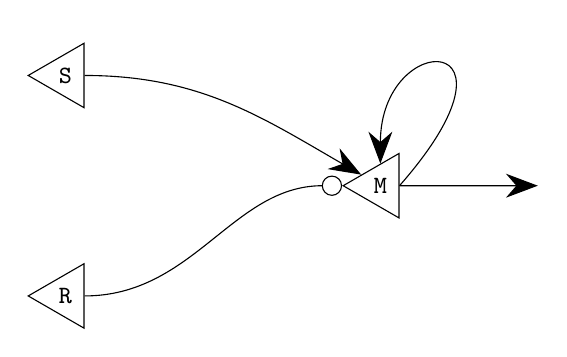
\begin{tikzpicture}
    [   neuron/.style=
        {   draw
        ,   regular polygon
        ,   regular polygon sides = 3
        ,   shape border rotate = 90
        ,   inner sep = 2pt
        ,   node font = \small\ttfamily
        }
    ,   baseline = 0pt
    ,   > = {Stealth[scale=2.4]}
    ]
    \node[neuron] (S) at (0cm, 14mm) {S};
    \node[neuron] (R) at (0cm,-14mm) {R};
    \node[neuron] (M) at (4cm, 0cm) {M};
    \draw[->] (S) to[out=0,in=150] (M);
    \draw[-{Circle[scale=2,open]}] (R) to[out=0,in=180] (M);
    \draw[->] (M.east) .. controls (6cm,2cm) and (4cm,2cm) .. (M);
    \draw[->] (M.east) to (6cm,0cm);
\end{tikzpicture}
}{%
            Example SR Flip-Flop using McCulloch's neurons.
        }
        Later, a concept called the perceptron was built by
        \cite{Rosenblatt:1958:Perceptron}.
        The perceptron consisted of a number of photovoltaic cells, which
        connected to a number of association cells, which then connected to a
        number of response cells.

        Each photovoltaic cell was connected to every association cell, and each
        association cell was connected to every response cell, this kind of
        connectivity is referred to a being densely connected.
        The output of each association cell was a boolean value based on the
        weighted sum of the input values, where the weights are automatically
        adjusted by the perceptron.
    \end{block}
    \vspace{1cm}
    \begin{block}{Modern Neural Networks}
        The most common architecture for artificial neurons was outlined by
        \cite{McClelland:1986:Parallel}, where the activation is given by
        \begin{align*}
            y_i = \phi\left(b_i + \sum_j w_{i,j}x_j\right),
        \end{align*}
        where $x_j$ is the $j^\text{th}$ input, $w_{i,j}$ is the connection
        weight from $j$ to $i$, $b_i$ is the input bias, and $\phi$ is some
        activation function.

        Learning is performed using a technique called backpropagation, which
        applies the chain rule to differentiate an value function with respect
        to each weight.
    \end{block}

\end{column}
\begin{column}[t]{0.3\textwidth}

    \begin{block}{Curve Fitting}
        An implementation of a neural network was written in python to predict
        the values of houses within Boston, based on three attributes:
        number of rooms, highway accessibility, and percentage of lower status
        population.
        The network consisted of three input neurons and one output neuron,
        using $\tanh$ as the activation function.
        \rfig[-1ex]{\begin{tikzpicture}
    \begin{axis}
        [   width = 0.8\textwidth
        ,   xtick = {1012,3036,5060}
        ,   ytick = {-0.3,-0.2,-0.1,0,0.1,0.2}
        ,   xmin = -200
        ,   xmax = 5260
        ,   legend pos = south west
        ,   xlabel = {Iteration}
        ,   ylabel = {Value}
        ]
        \addplot [color = Rblue]   table [col sep = comma]
        {../Code/BostonHousing/DataPythonSingleW0.csv};
        \addplot [color = Rorange] table [col sep = comma]
        {../Code/BostonHousing/DataPythonSingleW1.csv};
        \addplot [color = Rgreen]  table [col sep = comma]
        {../Code/BostonHousing/DataPythonSingleW2.csv};
        \addplot [color = Rred]    table [col sep = comma]
        {../Code/BostonHousing/DataPythonSingleW3.csv};
        \legend{$w_0$,$w_1$,$w_2$,$w_3$}

        \addplot
        [   opacity = 0.2
        ,   sharp plot
        ,   update limits = false
        ]   coordinates {(0,-1) (0,1)};
        \pgfplotsinvokeforeach{1,...,10}%
        {   \addplot
            [   opacity = 0.2
            ,   sharp plot
            ,   update limits = false
            ]   coordinates {(506*#1,-1) (506*#1,1)}
            node [anchor = south west, rotate = 90] at (506*#1,0.015)
            {\tiny Epoch: #1};
        }
    \end{axis}
\end{tikzpicture}
}{%
            Network weights against iteration number.
        }
    \end{block}
    \vspace{1cm}
    \begin{block}{Image Recognition}
        Creating neural networks in python can be repetitive without the use of
        a library.
        TensorFlow provides an easy-to-use framework for creating neural
        networks in python which includes a variety of options for layers,
        activation functions, and optimisers.

        For image recognition, it is advantageous to use convolutional layers,
        in which each neuron is connected to a small region of the previous
        layer, and all the neurons share the same weight scheme.
        A convolutional neural network was in python using TensorFlow to perform
        character recognition on the MNIST dataset, which contains a large
        number of handwritten numbers.
        The network also contained ``dropout'' layers, which prevent the network
        from over fitting.
        \rfig{\begin{tikzpicture}
    \loaddata{../Code/CharacterRecognition/PosterFigrFlat.txt}
    \foreach\posx/\posy/\pred/\cert/\actu in \loadeddata
    {   \pgfmathtruncatemacro{\indx}{5*\posy+\posx}
        \node[draw] (N\indx) at (5*\posx,0)
        {\includegraphics[width=25mm]{CRResults/img\indx}};
        \node (P\indx) at (N\indx.north) [anchor=south]
        {\scriptsize Predicted: \pred};
        \node (A\indx) at (P\indx.north) [anchor=south,outer sep=0,inner sep=0]
        {\scriptsize Was: \actu};
        \node (S\indx) at (N\indx.south) [anchor=north]
        {\scriptsize \ifnum \actu=\pred
                Correct
            \else
                \underline{\textbf{Incorrect}}
            \fi};
        \node (C\indx) at (S\indx.south) [anchor=north,outer sep=0,inner sep=0]
        {\scriptsize Certainty: \cert};
    }
\end{tikzpicture}
}{%
            Network predictions for MNIST dataset.
        }
    \end{block}

\end{column}
\begin{column}[t]{0.3\textwidth}

    \begin{block}{Deep Q-Learning}
        Neural networks can also be used to interact with systems.
        The basis for the method is an algorithm called Q-Learning
        \citep{Watkins:1989:Learning}, which uses the Bellman equation,
        \begin{align*}
            Q(s,a) \leftarrow Q(s,a)
            + \alpha (&r + \gamma\max_{a'}Q(s',a')\\ &- Q(s,a)),
        \end{align*}
        where $Q(s,a)$ is the estimated future reward of taking action $a$ from
        state $s$, $s'$ is the state after the action,  $r$ is the reward of
        taking the action, $\gamma$ is the discount rate, and $\alpha$ is the
        learning rate.
        These Q-values are stored in a table.

        Once trained, the action with the highest Q-value from a given state is
        the optimal choice.

        The Q-table can be replaced with a neural network, which is trained to
        match its output with the Bellman equation.
    \end{block}
    \vspace{1cm}

    \begin{block}{Policy Gradient}
        For many problems, a deterministic policy is not optimal, and a
        stochastic policy is required.
        \cite{Sutton:2000:Policy} introduced an algorithm for learning
        probabilities, which defined the policy gradient as
        \begin{align*}
            \frac{\partial\rho}{\partial\theta} = \sum_s d(s) \sum_a
            \frac{\partial\pi(s,a)}{\partial\theta}Q(s,a),
        \end{align*}
        where $\rho$ is the expect reward, $\pi$ is the policy, $\theta$ is the
        parameter vector of $\pi$, $d(s)$ is the state distribution, and
        $Q(s,a)$ is the state-action pair value.

        Policy gradients and Q-Learning can be combined to form Actor-Critic
        methods, which are the current state-of-the-art for reinforcement
        learning.
    \end{block}
    \vspace{1cm}

    \begin{block}{Bibliography}
        \renewcommand*{\bibfont}{\normalfont\scriptsize}
        \linespread{1}
        \printbibliography
    \end{block}
    \begin{tikzpicture}
        [   remember picture
        ,   overlay
        ]
        \fill[white]
            ($(current page.north west) + (388mm,-15cm)$)
            rectangle ++(10mm,-70cm);
    \end{tikzpicture}
    \vspace{2cm}
    Email: alexanderjjohnson@outlook.com
\end{column}
\end{columns}
\end{frame}
\end{document}
